% Options for packages loaded elsewhere
\PassOptionsToPackage{unicode}{hyperref}
\PassOptionsToPackage{hyphens}{url}
%
\documentclass[
  man]{apa6}
\usepackage{amsmath,amssymb}
\usepackage{lmodern}
\usepackage{iftex}
\ifPDFTeX
  \usepackage[T1]{fontenc}
  \usepackage[utf8]{inputenc}
  \usepackage{textcomp} % provide euro and other symbols
\else % if luatex or xetex
  \usepackage{unicode-math}
  \defaultfontfeatures{Scale=MatchLowercase}
  \defaultfontfeatures[\rmfamily]{Ligatures=TeX,Scale=1}
\fi
% Use upquote if available, for straight quotes in verbatim environments
\IfFileExists{upquote.sty}{\usepackage{upquote}}{}
\IfFileExists{microtype.sty}{% use microtype if available
  \usepackage[]{microtype}
  \UseMicrotypeSet[protrusion]{basicmath} % disable protrusion for tt fonts
}{}
\makeatletter
\@ifundefined{KOMAClassName}{% if non-KOMA class
  \IfFileExists{parskip.sty}{%
    \usepackage{parskip}
  }{% else
    \setlength{\parindent}{0pt}
    \setlength{\parskip}{6pt plus 2pt minus 1pt}}
}{% if KOMA class
  \KOMAoptions{parskip=half}}
\makeatother
\usepackage{xcolor}
\usepackage{graphicx}
\makeatletter
\def\maxwidth{\ifdim\Gin@nat@width>\linewidth\linewidth\else\Gin@nat@width\fi}
\def\maxheight{\ifdim\Gin@nat@height>\textheight\textheight\else\Gin@nat@height\fi}
\makeatother
% Scale images if necessary, so that they will not overflow the page
% margins by default, and it is still possible to overwrite the defaults
% using explicit options in \includegraphics[width, height, ...]{}
\setkeys{Gin}{width=\maxwidth,height=\maxheight,keepaspectratio}
% Set default figure placement to htbp
\makeatletter
\def\fps@figure{htbp}
\makeatother
\setlength{\emergencystretch}{3em} % prevent overfull lines
\providecommand{\tightlist}{%
  \setlength{\itemsep}{0pt}\setlength{\parskip}{0pt}}
\setcounter{secnumdepth}{-\maxdimen} % remove section numbering
% Make \paragraph and \subparagraph free-standing
\ifx\paragraph\undefined\else
  \let\oldparagraph\paragraph
  \renewcommand{\paragraph}[1]{\oldparagraph{#1}\mbox{}}
\fi
\ifx\subparagraph\undefined\else
  \let\oldsubparagraph\subparagraph
  \renewcommand{\subparagraph}[1]{\oldsubparagraph{#1}\mbox{}}
\fi
\newlength{\cslhangindent}
\setlength{\cslhangindent}{1.5em}
\newlength{\csllabelwidth}
\setlength{\csllabelwidth}{3em}
\newlength{\cslentryspacingunit} % times entry-spacing
\setlength{\cslentryspacingunit}{\parskip}
\newenvironment{CSLReferences}[2] % #1 hanging-ident, #2 entry spacing
 {% don't indent paragraphs
  \setlength{\parindent}{0pt}
  % turn on hanging indent if param 1 is 1
  \ifodd #1
  \let\oldpar\par
  \def\par{\hangindent=\cslhangindent\oldpar}
  \fi
  % set entry spacing
  \setlength{\parskip}{#2\cslentryspacingunit}
 }%
 {}
\usepackage{calc}
\newcommand{\CSLBlock}[1]{#1\hfill\break}
\newcommand{\CSLLeftMargin}[1]{\parbox[t]{\csllabelwidth}{#1}}
\newcommand{\CSLRightInline}[1]{\parbox[t]{\linewidth - \csllabelwidth}{#1}\break}
\newcommand{\CSLIndent}[1]{\hspace{\cslhangindent}#1}
\ifLuaTeX
\usepackage[bidi=basic]{babel}
\else
\usepackage[bidi=default]{babel}
\fi
\babelprovide[main,import]{english}
% get rid of language-specific shorthands (see #6817):
\let\LanguageShortHands\languageshorthands
\def\languageshorthands#1{}
% Manuscript styling
\usepackage{upgreek}
\captionsetup{font=singlespacing,justification=justified}

% Table formatting
\usepackage{longtable}
\usepackage{lscape}
% \usepackage[counterclockwise]{rotating}   % Landscape page setup for large tables
\usepackage{multirow}		% Table styling
\usepackage{tabularx}		% Control Column width
\usepackage[flushleft]{threeparttable}	% Allows for three part tables with a specified notes section
\usepackage{threeparttablex}            % Lets threeparttable work with longtable

% Create new environments so endfloat can handle them
% \newenvironment{ltable}
%   {\begin{landscape}\centering\begin{threeparttable}}
%   {\end{threeparttable}\end{landscape}}
\newenvironment{lltable}{\begin{landscape}\centering\begin{ThreePartTable}}{\end{ThreePartTable}\end{landscape}}

% Enables adjusting longtable caption width to table width
% Solution found at http://golatex.de/longtable-mit-caption-so-breit-wie-die-tabelle-t15767.html
\makeatletter
\newcommand\LastLTentrywidth{1em}
\newlength\longtablewidth
\setlength{\longtablewidth}{1in}
\newcommand{\getlongtablewidth}{\begingroup \ifcsname LT@\roman{LT@tables}\endcsname \global\longtablewidth=0pt \renewcommand{\LT@entry}[2]{\global\advance\longtablewidth by ##2\relax\gdef\LastLTentrywidth{##2}}\@nameuse{LT@\roman{LT@tables}} \fi \endgroup}

% \setlength{\parindent}{0.5in}
% \setlength{\parskip}{0pt plus 0pt minus 0pt}

% Overwrite redefinition of paragraph and subparagraph by the default LaTeX template
% See https://github.com/crsh/papaja/issues/292
\makeatletter
\renewcommand{\paragraph}{\@startsection{paragraph}{4}{\parindent}%
  {0\baselineskip \@plus 0.2ex \@minus 0.2ex}%
  {-1em}%
  {\normalfont\normalsize\bfseries\itshape\typesectitle}}

\renewcommand{\subparagraph}[1]{\@startsection{subparagraph}{5}{1em}%
  {0\baselineskip \@plus 0.2ex \@minus 0.2ex}%
  {-\z@\relax}%
  {\normalfont\normalsize\itshape\hspace{\parindent}{#1}\textit{\addperi}}{\relax}}
\makeatother

% \usepackage{etoolbox}
\makeatletter
\patchcmd{\HyOrg@maketitle}
  {\section{\normalfont\normalsize\abstractname}}
  {\section*{\normalfont\normalsize\abstractname}}
  {}{\typeout{Failed to patch abstract.}}
\patchcmd{\HyOrg@maketitle}
  {\section{\protect\normalfont{\@title}}}
  {\section*{\protect\normalfont{\@title}}}
  {}{\typeout{Failed to patch title.}}
\makeatother

\usepackage{xpatch}
\makeatletter
\xapptocmd\appendix
  {\xapptocmd\section
    {\addcontentsline{toc}{section}{\appendixname\ifoneappendix\else~\theappendix\fi\\: #1}}
    {}{\InnerPatchFailed}%
  }
{}{\PatchFailed}
\keywords{body position, motor development, everyday experiences, sitting, machine learning\newline\indent Word count: X}
\DeclareDelayedFloatFlavor{ThreePartTable}{table}
\DeclareDelayedFloatFlavor{lltable}{table}
\DeclareDelayedFloatFlavor*{longtable}{table}
\makeatletter
\renewcommand{\efloat@iwrite}[1]{\immediate\expandafter\protected@write\csname efloat@post#1\endcsname{}}
\makeatother
\usepackage{csquotes}
\raggedbottom
\ifLuaTeX
  \usepackage{selnolig}  % disable illegal ligatures
\fi
\IfFileExists{bookmark.sty}{\usepackage{bookmark}}{\usepackage{hyperref}}
\IfFileExists{xurl.sty}{\usepackage{xurl}}{} % add URL line breaks if available
\urlstyle{same} % disable monospaced font for URLs
\hypersetup{
  pdftitle={Full-day, in home validation of infant body position measurements from inertial sensors},
  pdfauthor={John M. Franchak1, Maximilian Tang1, Hailey Rousey1, \& Chuan Luo1},
  pdflang={en-EN},
  pdfkeywords={body position, motor development, everyday experiences, sitting, machine learning},
  hidelinks,
  pdfcreator={LaTeX via pandoc}}

\title{Full-day, in home validation of infant body position measurements from inertial sensors}
\author{John M. Franchak\textsuperscript{1}, Maximilian Tang\textsuperscript{1}, Hailey Rousey\textsuperscript{1}, \& Chuan Luo\textsuperscript{1}}
\date{}


\shorttitle{Infant position in the home}

\authornote{

Add complete departmental affiliations for each author here. Each new line herein must be indented, like this line.

Enter author note here.

Correspondence concerning this article should be addressed to John M. Franchak, UC Riverside Department of Psychology, 900 University Avenue, Riverside, CA 92521. E-mail: \href{mailto:franchak@ucr.edu}{\nolinkurl{franchak@ucr.edu}}

}

\affiliation{\phantom{0}}

\abstract{%
Abstract
}



\begin{document}
\maketitle

\hypertarget{current-study}{%
\section{Current Study}\label{current-study}}

\hypertarget{methods}{%
\section{Methods}\label{methods}}

\hypertarget{participants}{%
\subsection{Participants}\label{participants}}

\hypertarget{apparatus}{%
\subsection{Apparatus}\label{apparatus}}

\hypertarget{procedure}{%
\subsection{Procedure}\label{procedure}}

\begin{figure}

{\centering 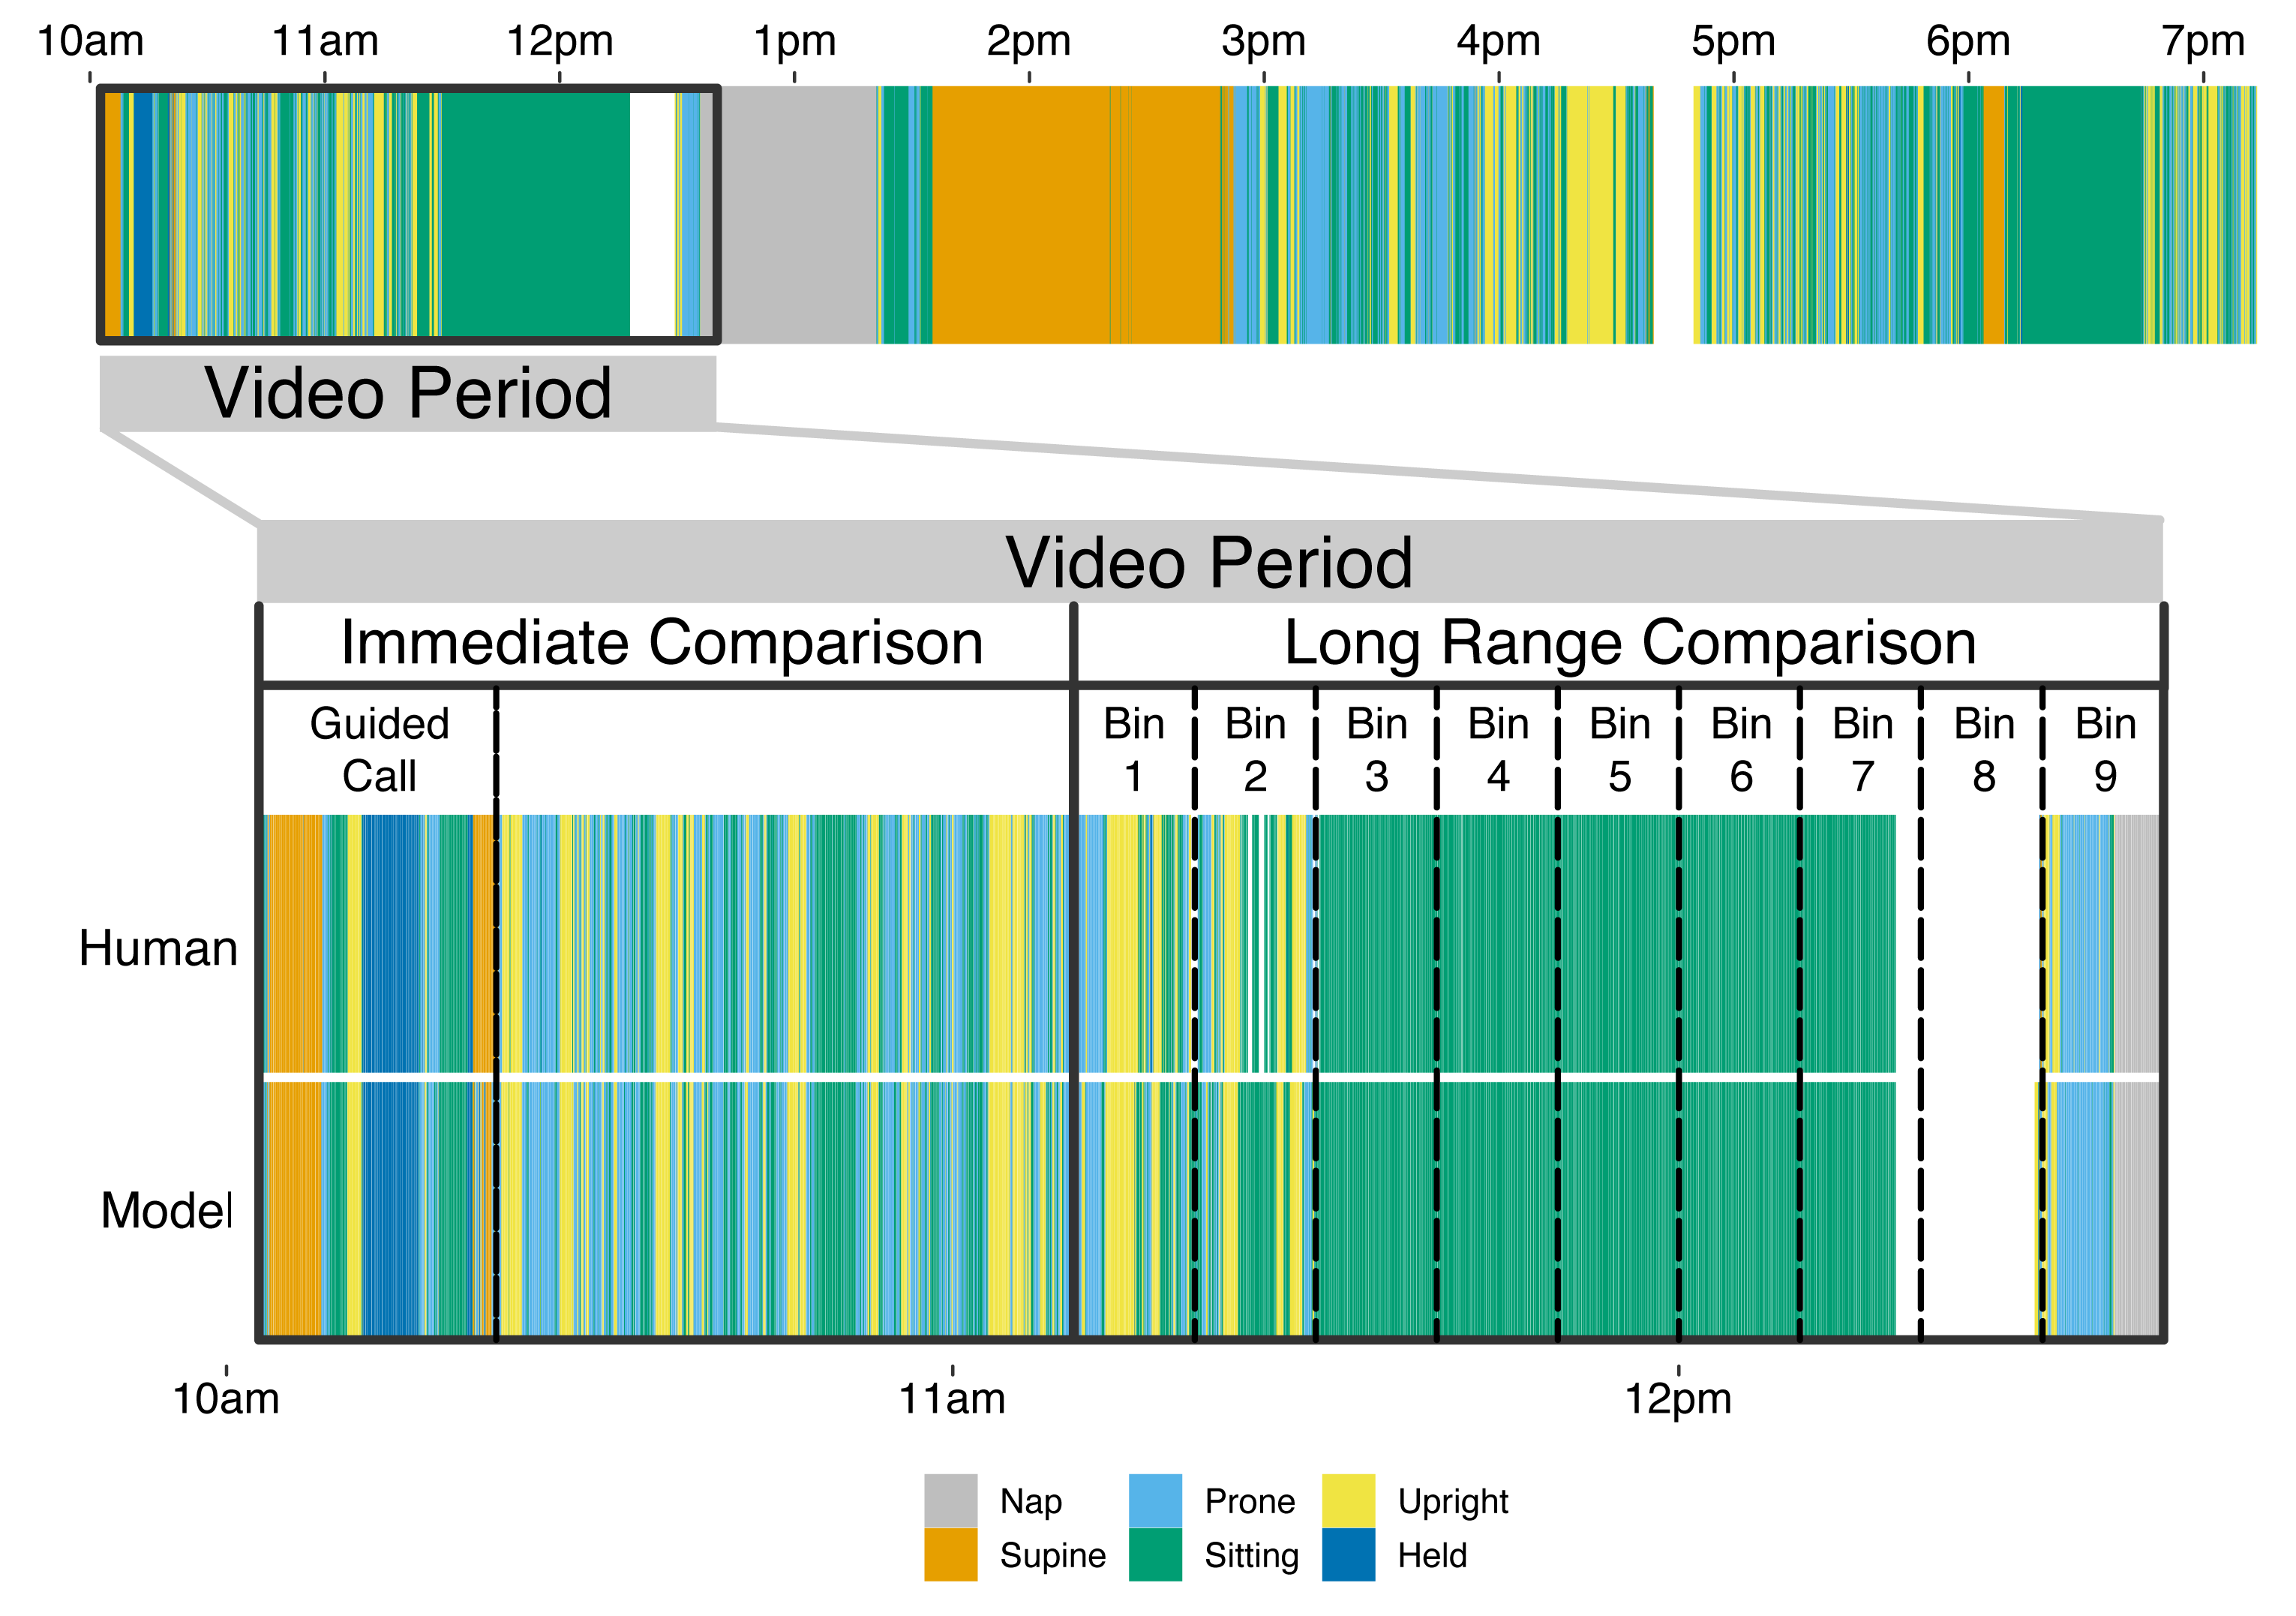
\includegraphics[width=0.9\linewidth]{figures/timeline} 

}

\caption{Example Timeline Caption.}\label{fig:exemplartimeline}
\end{figure}

\hypertarget{body-position-annotation}{%
\subsection{Body position annotation}\label{body-position-annotation}}

\hypertarget{body-position-classification}{%
\subsection{Body position classification}\label{body-position-classification}}

\hypertarget{results}{%
\section{Results}\label{results}}

\hypertarget{goal-1-optimize-and-validate-body-position-classification-model}{%
\subsection{Goal 1: Optimize and validate body position classification model}\label{goal-1-optimize-and-validate-body-position-classification-model}}

\begin{figure}

{\centering 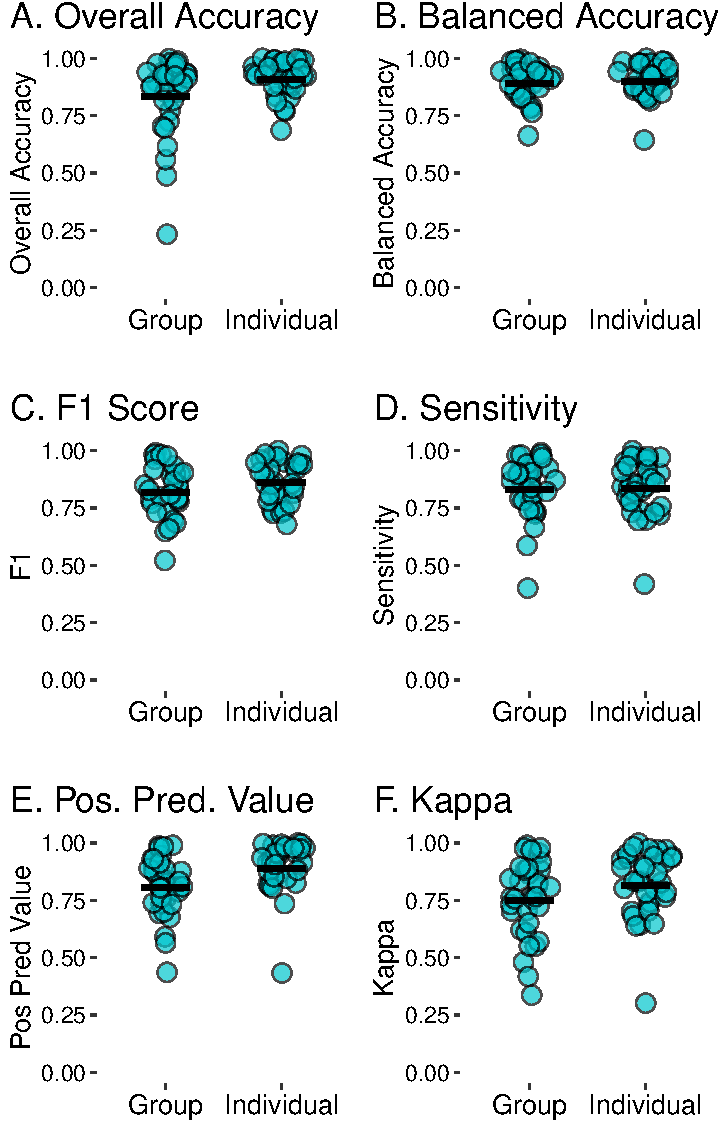
\includegraphics{manuscript_files/figure-latex/metrics-1} 

}

\caption{Metrics}\label{fig:metrics}
\end{figure}

\begin{table}[tbp]

\begin{center}
\begin{threeparttable}

\caption{\label{tab:metricstable}Summary statistics for model performance metrics shown separately for group and individual models.}

\begin{tabular}{lllllll}
\toprule
 & \multicolumn{3}{c}{Group} & \multicolumn{3}{c}{Individual} \\
\cmidrule(r){2-4} \cmidrule(r){5-7}
Metric & Median & Mean & SD & Median & Mean & SD\\
\midrule
Overall Accuracy & 0.908 & 0.848 & 0.143 & 0.936 & 0.919 & 0.071\\
Balanced Accuracy & 0.909 & 0.897 & 0.074 & 0.916 & 0.907 & 0.072\\
F1 & 0.813 & 0.827 & 0.101 & 0.873 & 0.870 & 0.089\\
Sensitivity & 0.840 & 0.836 & 0.123 & 0.848 & 0.840 & 0.121\\
Pos Pred Value & 0.822 & 0.815 & 0.125 & 0.915 & 0.899 & 0.108\\
Kappa & 0.769 & 0.757 & 0.160 & 0.846 & 0.820 & 0.141\\
\bottomrule
\end{tabular}

\end{threeparttable}
\end{center}

\end{table}

\renewcommand{\arraystretch}{.75}

\begin{table}[tbp]

\begin{center}
\begin{threeparttable}

\caption{\label{tab:metricsbyclass}Summary statistics for model performance metrics shown separately for group and individual models.}

\begin{tabular}{llllllll}
\toprule
 &  & \multicolumn{3}{c}{Group} & \multicolumn{3}{c}{Individual} \\
\cmidrule(r){3-5} \cmidrule(r){6-8}
Metric & Position & Median & Mean & SD & Median & Mean & SD\\
\midrule
Balanced Accuracy & Supine & 0.977 & 0.935 & 0.099 & 0.995 & 0.957 & 0.090\\
 & Prone & 0.997 & 0.950 & 0.110 & 0.983 & 0.921 & 0.132\\
 & Sitting & 0.932 & 0.861 & 0.151 & 0.973 & 0.943 & 0.071\\
 & Upright & 0.930 & 0.867 & 0.146 & 0.937 & 0.877 & 0.123\\
 & Held & 0.907 & 0.872 & 0.111 & 0.892 & 0.854 & 0.153\\ \midrule
F1 & Supine & 0.952 & 0.873 & 0.173 & 0.987 & 0.937 & 0.130\\
 & Prone & 0.965 & 0.923 & 0.124 & 0.958 & 0.889 & 0.186\\
 & Sitting & 0.897 & 0.805 & 0.247 & 0.963 & 0.927 & 0.101\\
 & Upright & 0.781 & 0.748 & 0.235 & 0.868 & 0.769 & 0.227\\
 & Held & 0.813 & 0.783 & 0.163 & 0.862 & 0.786 & 0.240\\ \midrule
Sensitivity & Supine & 1.000 & 0.945 & 0.125 & 1.000 & 0.948 & 0.141\\
 & Prone & 1.000 & 0.907 & 0.216 & 0.988 & 0.856 & 0.266\\
 & Sitting & 0.901 & 0.787 & 0.291 & 0.977 & 0.917 & 0.136\\
 & Upright & 0.878 & 0.767 & 0.275 & 0.893 & 0.790 & 0.255\\
 & Held & 0.867 & 0.774 & 0.229 & 0.817 & 0.722 & 0.309\\ \midrule
Pos Pred Value & Supine & 0.973 & 0.802 & 0.300 & 1.000 & 0.939 & 0.131\\
 & Prone & 0.991 & 0.896 & 0.196 & 0.993 & 0.901 & 0.197\\
 & Sitting & 0.910 & 0.840 & 0.238 & 0.967 & 0.947 & 0.078\\
 & Upright & 0.848 & 0.743 & 0.285 & 0.875 & 0.817 & 0.205\\
 & Held & 0.917 & 0.803 & 0.247 & 0.949 & 0.872 & 0.232\\ \midrule
Kappa & Supine & 0.932 & 0.770 & 0.307 & 0.984 & 0.913 & 0.169\\
 & Prone & 0.951 & 0.887 & 0.208 & 0.948 & 0.851 & 0.242\\
 & Sitting & 0.836 & 0.712 & 0.308 & 0.946 & 0.889 & 0.134\\
 & Upright & 0.729 & 0.700 & 0.277 & 0.829 & 0.744 & 0.232\\
 & Held & 0.786 & 0.733 & 0.219 & 0.845 & 0.744 & 0.280\\
\bottomrule
\end{tabular}

\end{threeparttable}
\end{center}

\end{table}

\hypertarget{goal-2-assess-classification-accuracy-over-long-recordings}{%
\subsection{Goal 2: Assess classification accuracy over long recordings}\label{goal-2-assess-classification-accuracy-over-long-recordings}}

\begin{figure}

{\centering 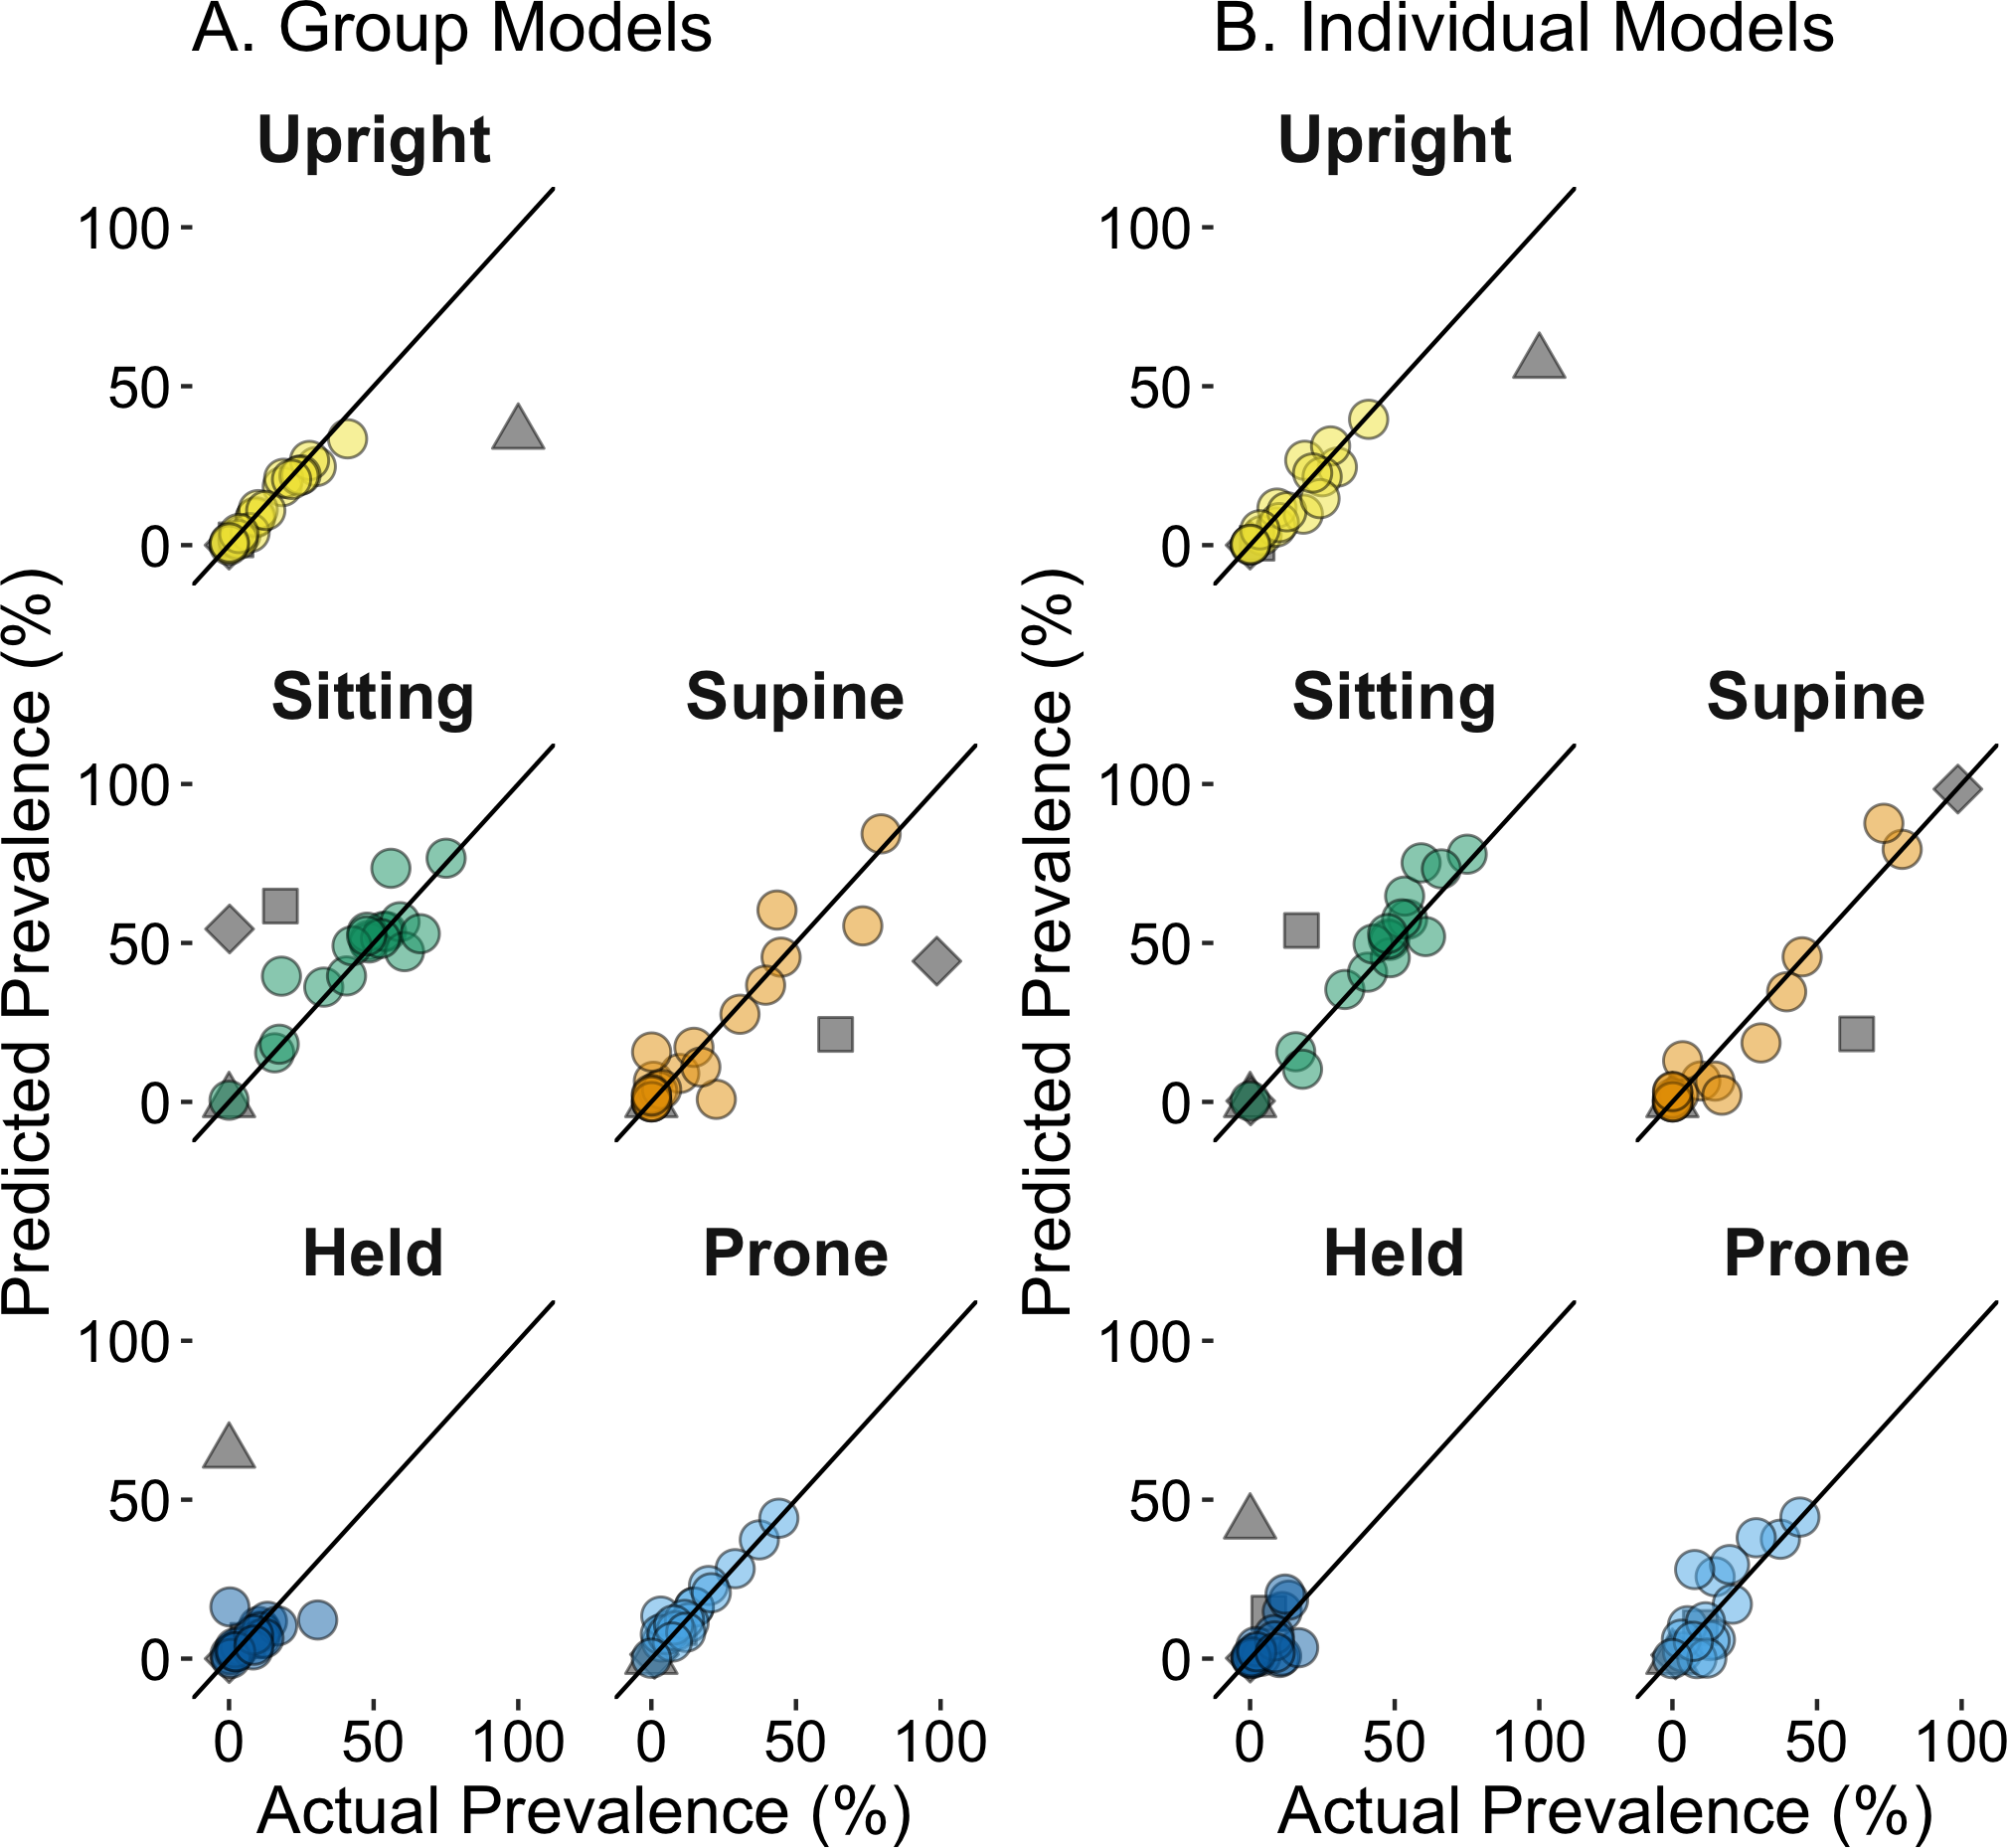
\includegraphics{manuscript_files/figure-latex/part2overall-1} 

}

\caption{Overall agreement between human-coded body position and model-predicted body position in the long-delay period. Agreement for group models is shown in (A) and agreement for individual models is shown in (B). Plots are shown separately for each body position with a reference line that indicates perfect agreement; each point in a plot represent data for a single participant. The three outlier participants are plotted in dark gray, with a different shape marking each individual.}\label{fig:part2overall}
\end{figure}

\begin{table}[tbp]

\begin{center}
\begin{threeparttable}

\caption{\label{tab:pt2overalltable}Correlations between human-coded and model-predicted body position durations across the entire long delay period. Correlations are provided within each posture and overall, and computed separately using group and individual models with and without outlier participants.}

\begin{tabular}{lllll}
\toprule
 & \multicolumn{2}{c}{With Outliers} & \multicolumn{2}{c}{Without Outliers} \\
\cmidrule(r){2-3} \cmidrule(r){4-5}
Position & Group & Individual & Group & Individual\\
\midrule
Held & -0.02 & 0.16 & 0.55 & 0.63\\
Prone & 0.97 & 0.83 & 0.97 & 0.84\\
Sitting & 0.72 & 0.93 & 0.91 & 0.97\\
Supine & 0.84 & 0.93 & 0.94 & 0.97\\
Upright & 0.84 & 0.93 & 0.99 & 0.94\\ \midrule
Overall & 0.79 & 0.90 & 0.95 & 0.96\\
\bottomrule
\end{tabular}

\end{threeparttable}
\end{center}

\end{table}

\begin{figure}

{\centering 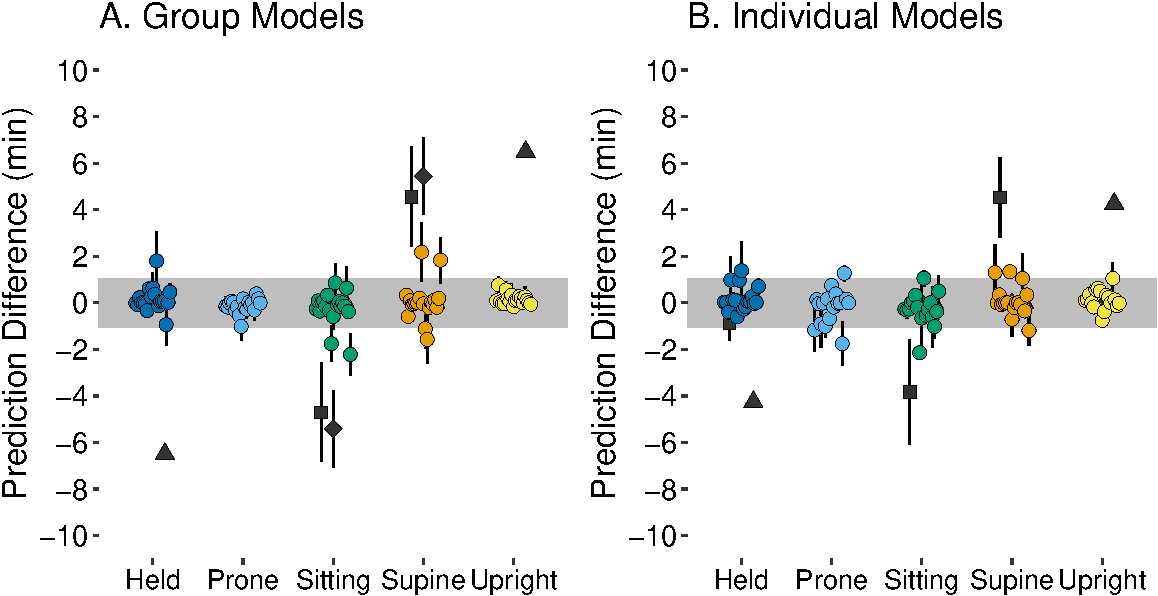
\includegraphics{manuscript_files/figure-latex/part2bins-1} 

}

\caption{Prediction performance (difference in minutes between human-coded and model-predicted body position) for 10-minute bins in the long delay period. Each point shows the mean and SE for a single participant for each body position, summarizing the prediction difference for each of their 10-minute bins. Points falling within the gray shaded region indicate that average prediction errors were less than 1 minute. Performance is plotted separately for (A) group models and (B) individual models. The three outlier participants are plotted in dark gray, with a different shape marking each individual.}\label{fig:part2bins}
\end{figure}

\begin{table}[tbp]

\begin{center}
\begin{threeparttable}

\caption{\label{tab:pt2binstable}Correlations between human-coded and model-predicted body position durations using 10-minute bins during the long delay period. Correlations are provided within each posture and overall, and computed separately using group and individual models with and without outlier participants.}

\begin{tabular}{lllll}
\toprule
 & \multicolumn{2}{c}{With Outliers} & \multicolumn{2}{c}{Without Outliers} \\
\cmidrule(r){2-3} \cmidrule(r){4-5}
Position & Group & Individual & Group & Individual\\
\midrule
Held & 0.45 & 0.44 & 0.57 & 0.56\\
Prone & 0.96 & 0.81 & 0.96 & 0.88\\
Sitting & 0.72 & 0.93 & 0.91 & 0.93\\
Supine & 0.75 & 0.93 & 0.90 & 0.94\\
Upright & 0.93 & 0.95 & 0.97 & 0.95\\ \midrule
Overall & 0.80 & 0.92 & 0.92 & 0.94\\
\bottomrule
\end{tabular}

\end{threeparttable}
\end{center}

\end{table}

\hypertarget{goal-3-examine-wear-time-and-compliance-in-full-day-data-collection}{%
\subsection{Goal 3: Examine wear time and compliance in full-day data collection}\label{goal-3-examine-wear-time-and-compliance-in-full-day-data-collection}}

\begin{figure}

{\centering 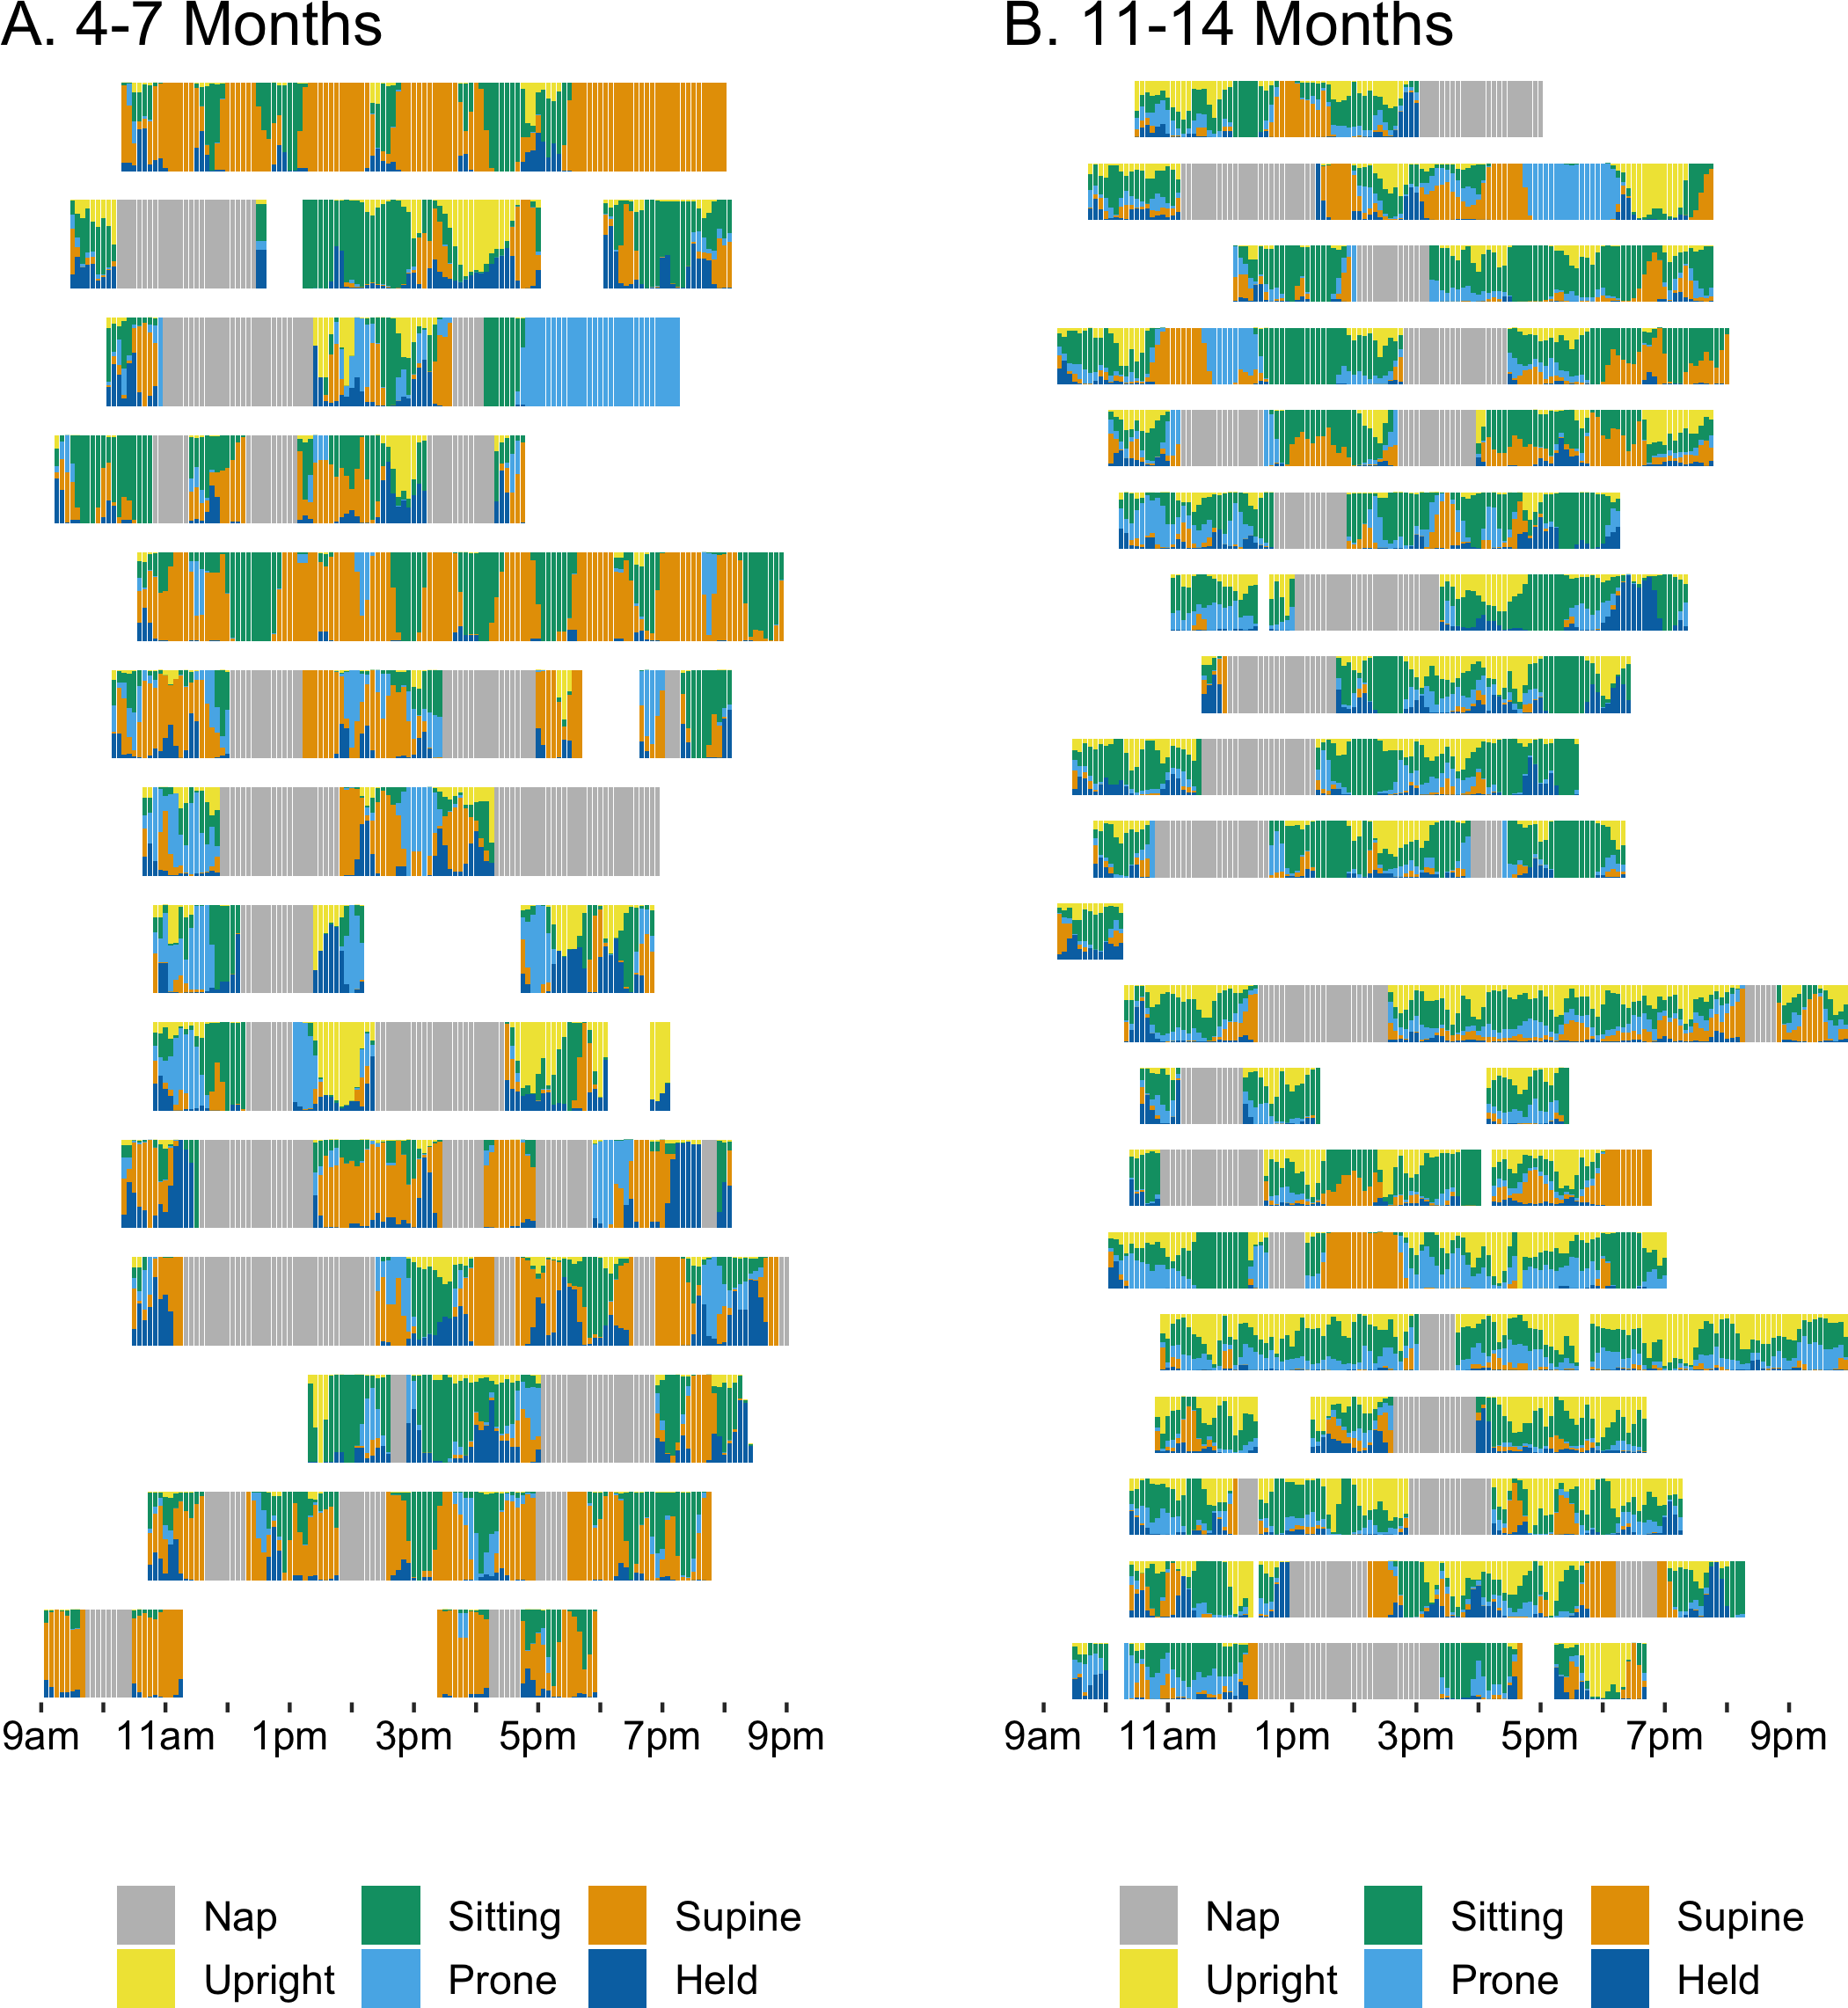
\includegraphics{manuscript_files/figure-latex/timelines-1} 

}

\caption{Timelines}\label{fig:timelines}
\end{figure}

\hypertarget{goal-4-determine-sensitivity-of-classification-to-measure-age-differences-in-body-position}{%
\subsection{Goal 4: Determine sensitivity of classification to measure age differences in body position}\label{goal-4-determine-sensitivity-of-classification-to-measure-age-differences-in-body-position}}

\begin{figure}

{\centering 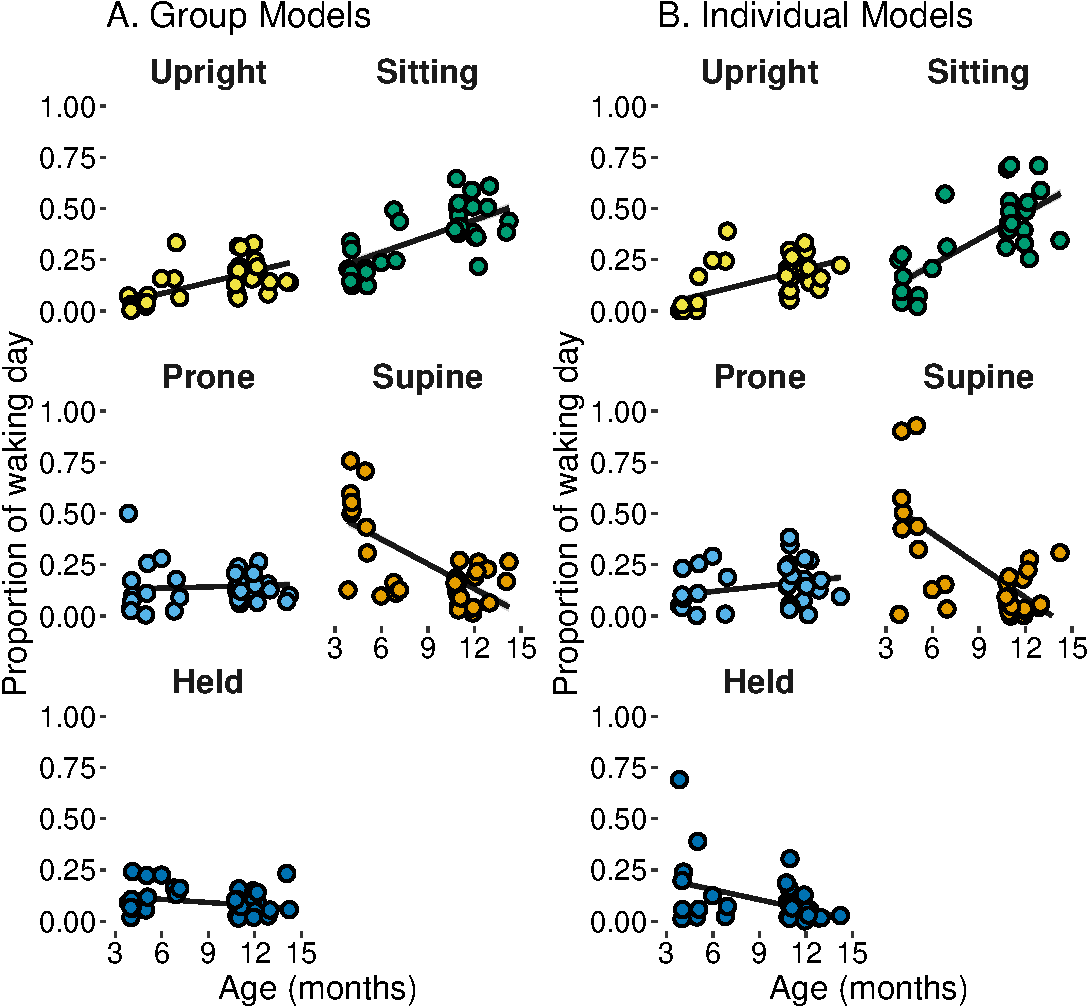
\includegraphics{manuscript_files/figure-latex/age-1} 

}

\caption{Age trends}\label{fig:age}
\end{figure}

\begin{table}[tbp]

\begin{center}
\begin{threeparttable}

\caption{\label{tab:agetable}Summary of age differences in full-day body position for younger (4- to 7-month) and older (11- to 14-month) infants. Values shown are the mean percent of time for each body position averaged across infants in each group. Standard deviations are shown in parentheses. Descriptive statistics are shown separately for group and individual models.}

\begin{tabular}{lllll}
\toprule
 & \multicolumn{2}{c}{Group} & \multicolumn{2}{c}{Individual} \\
\cmidrule(r){2-3} \cmidrule(r){4-5}
Position & Younger & Older & Younger & Older\\
\midrule
Upright & 7.6\% (8.9) & 18.6\% (7.4) & 9.9\% (13.1) & 18.7\% (8.4)\\
Sitting & 26.3\% (12.1) & 44.4\% (10.1) & 20.2\% (16.3) & 46.9\% (13.3)\\
Prone & 13.8\% (13.5) & 14.4\% (6.0) & 11.9\% (9.9) & 16.9\% (10.6)\\
Supine & 37.9\% (23.2) & 14.0\% (8.4) & 39.4\% (30.3) & 10.0\% (9.5)\\
Held & 12.7\% (6.9) & 8.5\% (5.4) & 17.6\% (19.9) & 7.4\% (7.6)\\
\bottomrule
\end{tabular}

\end{threeparttable}
\end{center}

\end{table}

\hypertarget{discussion}{%
\section{Discussion}\label{discussion}}

\newpage

\hypertarget{references}{%
\section{References}\label{references}}

\hypertarget{refs}{}
\begin{CSLReferences}{0}{0}
\end{CSLReferences}


\end{document}
